\chapter{Síťová komunikace a databáze} \label{chap:network_database}
Smyslem zkonstruovaných čidel je jejich snadná implementace do bytu či domu. Senzory potřebují kabelově připojit jen napájení a celá komunikace mezi mikročipy a brokerem probíhá po WiFi. Tato schopnost bezdrátové komunikace zásadně rozšiřuje možnosti rozmístění senzorů po domácnosti. Komunikace senzorů se serverem využívá principů \textit{IoT} a síťový protokol \textit{MQTT}. 

\section*{Síť IoT} \label{sec:iot}
Síť IoT\footnote{\textbf{I}nternet \textbf{o}f \textbf{T}hings - internet věcí} je architektura na bázi internetu, která obecně slouží ke komunikaci a výměně dat. Senzory v projektu chytré domácnosti spadají do komponent v internetu věcí, protože veškerá komunikace probíhá po internetu a výhradně bez účasti uživatele. Technologie pro chytrou domácnost v tomto projektu byla navržena tak, aby uživatel měl přísun aktuálních dat ze senzorů bez nutnosti znalosti principů fungování celého systému. \par
Na \cref{fig:network_database_schema} se nachází diagram, na kterém je zobrazen přehled všech komponent, jejich propojení a datové toky v celém projektu. Červenými šipkami jsou znázorněny datové toky, které probíhají v reálném čase. V cloudové části je zálohována databáze a jelikož je cloudový počítač výkonnější než Raspberry Pi, může být využitý k trénování modelů, které jsou pak jednorázově při načtení webu nahrány do RPi. Samotné modely mohou být trénovány i přímo na RPi, ale proces trénování modelů všech měřených veličin trvá déle. Komunikace mezi RPi a frontendem webu je popsána v \cref{sec:websocket}.

\begin{figure}[H]
  \centering
  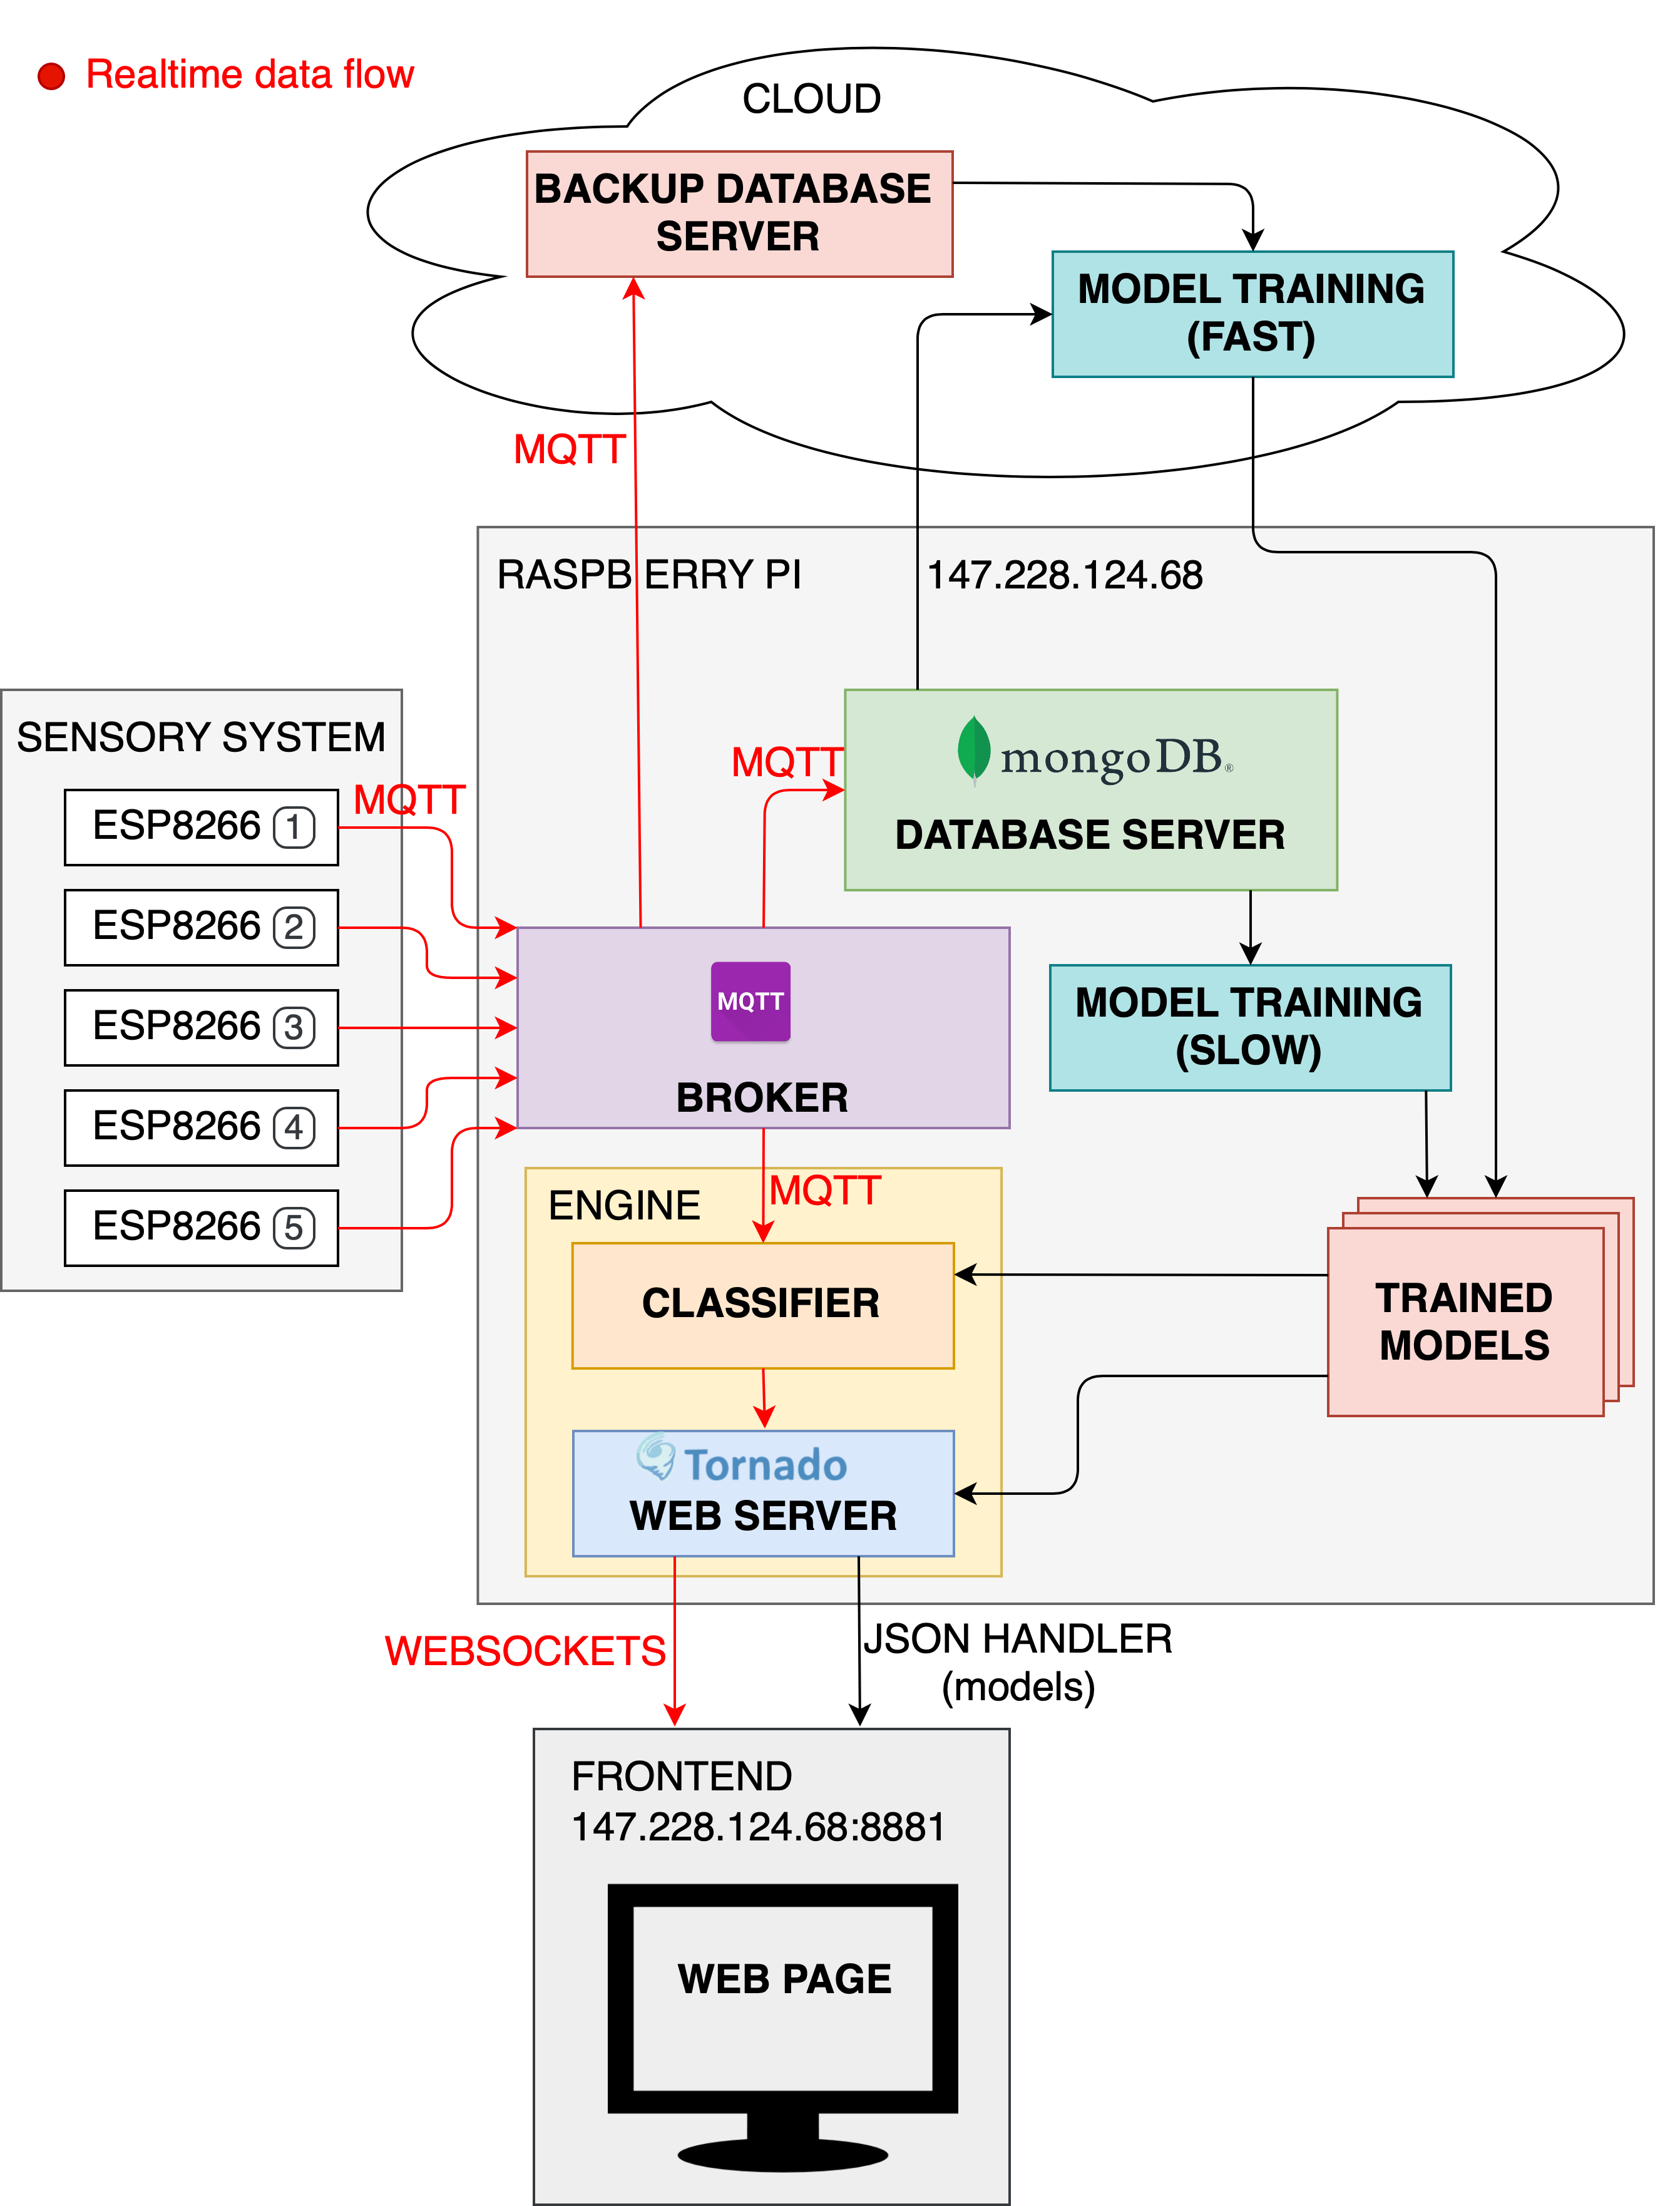
\includegraphics[width=0.8 \textwidth]{network_database_schema.png}
  \caption{Rozložení jednotlivých komponent a schéma datových toků v celém projektu}
  \label{fig:network_database_schema}
\end{figure}

\section{Protokol MQTT} \label{sec:protocol_mqtt}
MQTT\footnote{\textbf{M}essage \textbf{Q}ueuing \textbf{T}elemetry \textbf{T}ransport} je internetový protokol, který slouží k výměně zpráv mezi subjekty v síti. Tento protokol vznikl už v roce 1999, ale k významnému využití dochází i v dnešní době díky IoT aplikacím. MQTT pracuje na TCP/IP vrstvě a hodí se především v aplikacích, které vyžadují minimální datový přenos po síti.  \par
Při komunikaci prostřednictvím MQTT protokolu jsou v síti definovány dva typy entit - server a klient. V síti se nachází jeden server - \textit{broker} a libovolné množství klientů. Veškerá komunikace probíhá prostřednictvím brokeru. Broker je centrální místo v síti, na které ostatní zařízení publikují zprávy a který ostatním subjektům v síti umožňuje číst tyto zprávy. Klientem může být jakékoliv zařízení, které má přístup na internet a podporu MQTT protokolu. Zpravidla jde o chytré senzory, které publikují zprávy. V tomto projektu je broker spuštěn na počítači Raspberry Pi (více v \cref{sec:raspberry_pi}) a jako klienti figurují jednotlivé senzory - mikročipy ESP8266. Princip protokolu MQTT je zobrazen na \cref{fig:mqtt_communication}. Jednotlivé senzory publikují zprávy na broker (mód \textit{publish}) a broker přijímá všechny příchozí zprávy. Další aplikace jako je webový a databázový server odebírají příchozí zprávy od brokeru (mód \textit{subscribe}) za účelem dalšího zpracování dat. Z hlediska protokolu může být jeden klient současně \textit{publisher} i \textit{subscriber}, ale často bývají tyto role rozděleny. \textit{Publisher} je zpravidla senzor, který měří určitou fyzikální veličinu a hodnoty odesílá na broker. \textit{Subscriber} je většinou zařízení, které čte data zaslaná od \textit{publishera} a s těmito daty pak dále pracuje (například je zobrazuje ve webovém rozhraní nebo ukládá do databáze).  

\begin{figure}[H]
  \centering
  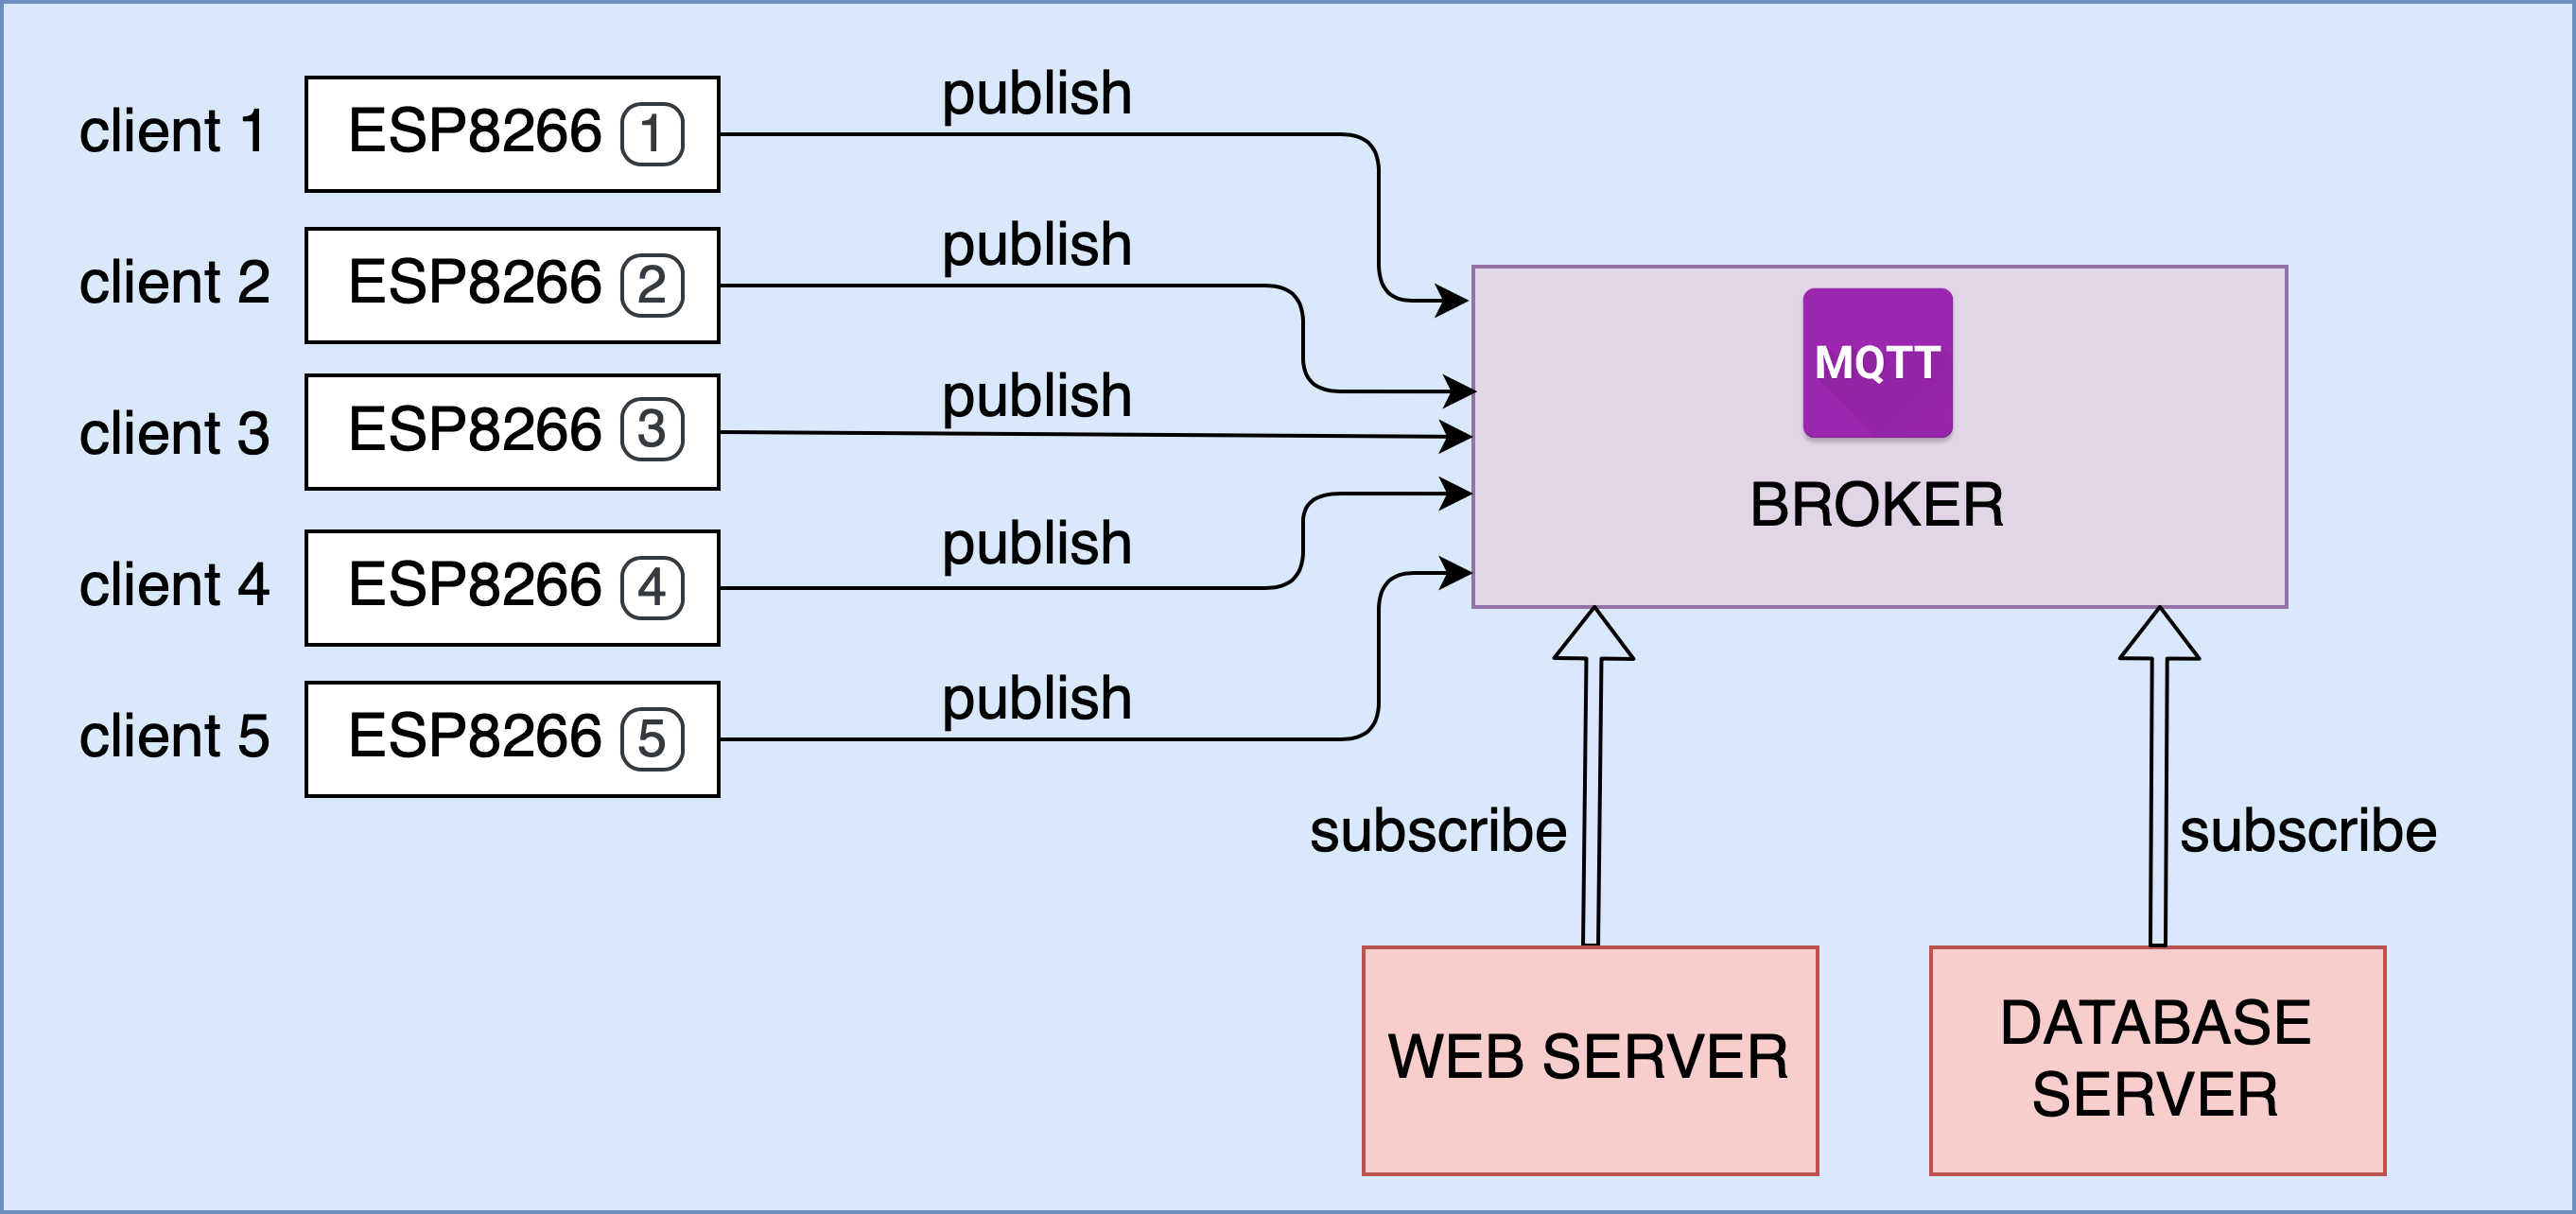
\includegraphics[width=0.7 \textwidth]{mqtt_diagram.png}
  \caption{Princip komunikace přes MQTT protokol}
  \label{fig:mqtt_communication}
\end{figure}

\subsection*{Bezpečnost přenosu dat}
Identifikace klienta probíhá prostřednictvím uživatelského jména a hesla. Přes protokol MQTT se přenášejí textové řetězce v kódování UTF-8, které ve výchozím stavu bez použití SSL\footnote{\textbf{S}ecure \textbf{S}ockets \textbf{L}ayer - šifrovací protokol mezi transportní a aplikační vrstvou} nejsou nijak šifrované. Na TCP portu 1883 používá protokol nešifrovanou komunikaci, která se hodí pro přenos necitlivých dat. Alternativně lze na přednastaveném portu 8883 použít přenos šifrovaný protokolem SSL. Jelikož v projektu chytré domácnosti jsou senzory i broker na místní domácí síti a nepřenášejí se citlivá data, komunikace není šifrována.

\subsection{Struktura zpráv} \label{subsec:message_structure}
Pomocí protokolu MQTT je možné odesílat libovolné formáty dat s omezením na maximální velikost jedné zprávy 256 MB. Senzory odesílají na broker zprávy v datovém formátu \textit{JSON}\footnote{\textbf{J}ava\textbf{S}cript \textbf{O}bject \textbf{N}otation - JavaScriptový objektový zápis}. Tento objektový formát umožňuje vytvářet hierarchické struktury zpráv ve formě řetězce znaků. JSON byl zvolen pro svou jednoduchost a přehlednost. Formát dat je pro člověka čitelný a výsledná zpráva je datově úsporná, tudíž vhodná pro pravidelné přenášení po síti bez zbytečného zvětšování datového toku. Níže je uvedena obecná struktura zprávy ve formátu JSON a jeden konkrétní příklad zprávy ze senzoru s vlhkostním čidlem. \\

\begin{lstlisting}[language=json]
{ "sensor_id": string
  "location": string
  "owner": string
  "status": string
  "quantity": string
  "value": float
  "timestamp": string }
\end{lstlisting}
\begin{lstlisting}[language=json]
{ "sensor_id": "dht11_01", 
  "location": "room", 
  "owner": "pn", 
  "status": "ok", 
  "quantity": "humidity", 
  "value": 46.0, 
  "timestamp": "2020-04-09 11:32:30" }
\end{lstlisting}

Obsah zprávy je uzavřen do složených závorek a zpráva se skládá z dvojic klíč-hodnota, kde klíčem je vždy první řetězec znaků ve dvojici (\textit{location}, \textit{owner}, atd.) a hodnota je řetězec znaků za dvojtečkou. Jednotlivé páry klíč-hodnota jsou od sebe odděleny čárkou. Každá zpráva se skládá z následujících atributů.

\begin{itemize}
  \item \textit{location} je atribut udávající umístění senzoru; Může nabývat hodnot \textit{room} v případě, že je senzor v místnosti nebo \textit{outside} u senzoru, který je venku.
  \item \textit{owner} udává provozovatele senzoru; Tento atribut slouží k filtraci senzorů podle majitele a využití má v případě, že je v jedné síti větší množství senzorů od různých vývojářů.
  \item \textit{status} nabývá obecně dvou hodnot - \textit{ok} nebo \textit{error}; Senzor posílá v každé zprávě status čidla, ze kterého načítá data o měřené veličině; Tento atribut má význam při automatické detekci chyb na úrovni mikročipu ESP8266 (více v \cref{sec:error_detection_esp}). 
  \item \textit{sensor\_id} je unikátní identifikátor, který se vztahuje přímo k danému čidlu; Například senzor obsluhující současně teplotní čidlo \textit{ds18b20} a vlhkostní čidlo \textit{dht11} má pro každé čidlo samostatný identifikátor - \textit{ds18b20\_01} a \textit{dht11\_01}. 
  \item \textit{quantity} je atribut popisující měřenou fyzikální veličinu; Význam tohoto atributu je v identifikaci měřené veličiny, protože senzory posílají hodnoty veličin bez jejich fyzikálních jednotek.  
  \item \textit{timestamp} je časová známka, která je přiložena ke každé zprávě a její hodnotou je okamžik odeslání zprávy; Jelikož časová synchronizace je řešena na úrovni samotného mikročipu, je možné ke každé zprávě přidávat časovou známku a díky tomu snadno filtrovat příchozí zprávy podle času a data, čímž odpadá problematika určování pořadí zpráv na brokeru.   
  \item \textit{value} je atribut, ve kterém se přenáší hodnota měřené fyzikální veličiny; Jde vždy o číselnou hodnotu bez jednotky; Například u senzoru měřícího teplotu může mít atribut hodnotu 25,3; U senzoru monitorujícího pohyb v místnosti nabývá atribut value hodnoty 1 nebo 0.  
\end{itemize}

V \cref{tab:mqtt_msg_structure} je po řádcích zobrazen výčet všech kombinací hodnot atributů, kterých mohou zprávy v projektu chytré domácnosti nabývat.  

\newpage

\begin{table}[h]
\centering
 \begin{tabular}{|c|c|c|c|c|c|c|} 
 \hline
  location & owner & status\footnotemark & sensor\_id & quantity  \\
 \hline\hline
 room & pn & ok & ds18b20\_01 & temperature \\ 
 outside & pn & ok & ds18b20\_02 & temperature \\
 room & pn & ok & dht11\_01 & humidity \\
 room & pn & ok & tsl2591\_01 & illuminance \\
 room & pn & ok & bme280\_01 & pressure \\
 room & pn & ok & bme280\_01 & temperature \\
 room & pn & ok & am312\_01 & motion \\
 room & pn & ok & ls311b38\_01 & door\_open \\
 room & pn & ok & ls311b38\_02 & window\_open \\
 \hline
 \end{tabular}
 \caption{Atributy zprávy odesílané z mikročipu na broker}
 \label{tab:mqtt_msg_structure}
\end{table}

\footnotetext{Hodnota atributu \textit{status} se může samozřejmě změnit z \textit{ok} na \textit{error}. Hodnoty atributů \textit{timestamp} a \textit{value} jsou logicky v každé zprávě jiné, proto nejsou uvedeny v tabulce.}

\subsection{Hierarchie zpráv} \label{subsec:message_hierarchy}
Při přenosu dat dochází k datovému toku ve směru od senzorů na broker. Broker pouze přijímá všechny zprávy, ale sám neposílá žádná data senzorům. Kvůli přehlednosti a jednotné struktuře posílaných zpráv je definována jasná hierarchie zpráv. Zprávy jsou odesílány do \textit{topiců}. Topic určuje téma dané zprávy a slouží k oddělení zpráv podle toho, od jakého odesílatele pocházejí, jakou fyzikální veličinu popisují a kde jsou měřené (v místnosti nebo venku). Každá zpráva je přiřazena právě jednomu tématu a název tohoto tématu určuje sám odesílatel zprávy. Příjemce zprávy pak jen musí znát název tématu, do kterého odesílatel publikuje zprávy. Témata jsou řetězce v kódování UTF-8 oddělená lomítky a jejich hierarchie není samotným protokolem nijak určená. Při návrhu hierarchie témat v projektu senzorického řešení domácnosti byl kladen důraz na univerzálnost a přirozenost s možností snadného rozšíření v budoucnu. \par
Základem názvů všech témat je slovo \textit{smarthome} označující název projektu. Za tímto slovem se přidá umístění senzoru a název měřené veličiny. Po spojení těchto třech slov vzniká název konkrétního topicu, kam senzor odesílá zprávy. V \cref{tab:mqtt_topic_structure} je uveden výčet všech topiců používaných v této práci.

\begin{table}[h]
\centering
 \begin{tabular}{|p{6cm}|} 
 \hline
  smarthome/<location>/<quantity>  \\
 \hline\hline
 smarthome/room/temperature \\ 
 smarthome/outside/temperature \\
 smarthome/room/humidity \\
 smarthome/room/illuminance \\
 smarthome/room/pressure \\
 smarthome/room/motion \\
 smarthome/room/door\_open \\
 smarthome/room/window\_open \\
 \hline
 \end{tabular}
 \caption{Výčet všech topiců, do kterých jsou odesílány zprávy}
 \label{tab:mqtt_topic_structure}
\end{table}

Hierarchie témat byla navržena tak, aby každá měřená fyzikální veličina měla svůj topic v závislosti na umístění. Díky této volbě je možné strukturu témat snadno rozšířit jak z hlediska lokalit (přidání dalších pokojů v chytré domácnosti - \textit{livingroom}, \textit{bedroom}, atd.), tak z hlediska veličin (například \textit{smoke\_detection}). Tento model hierarchie topiců také umožňuje spojovat témata do souvisejících celků. K těmto účelům slouží znaky + a \#. Symbol + nahrazuje jednu úroveň v topicu, pro odebírání například všech teplot nezávisle na lokaci nebo čidlu lze použít příkaz \textit{smarthome/+/temperature}. Symbol  \# nahrazuje slovo za posledním lomítkem, pro odebírání například všech veličin, které jsou měřeny v místnosti lze použít příkaz \mbox{\textit{smarthome/room/\#}}. 

\section{Ukládání dat do databáze} \label{sec:database}
Jelikož senzory v této práci odesílají zprávy velmi často - s periodou jedné minuty, je potřeba data vhodným způsobem ukládat. K tomu slouží datová základna (databáze), ve které jsou data s pevnou strukturou záznamů propojena pomocí klíčů a která umožňuje snadno filtrovat záznamy podle zadaných kritérií. V tomto projektu jsou data ukládána do \mbox{databáze \textit{MongoDB}}.

\subsection*{MongoDB}
MongoDB je multiplatformní dokumentová databáze, která na rozdíl od relačních databází využívajících systém tabulek, ukládá data do kolekcí - souborů, které jsou podobné formátu JSON. Tato databáze je pro projekt chytré domácnosti vhodná právě díky tomu, že nevyužívá klasický přístup ukládání dat do tabulek. Jednou z hlavních výhod klasických relačních databází je možnost provázat tabulky mezi sebou pomocí klíčů. To se hodí zpravidla na obsáhlejší záznamy, které je potřeba strukturovat a pomocí cizích klíčů provazovat s ostatními tabulkami. Data získaná ze senzorů mají jednotnou strukturu a ukládání do tabulek by bylo neefektivní, proto byla zvolena databáze MongoDB, která je pro archivaci tohoto typu dat vhodnější. Databáze MongoDB má širokou podporu programovacích jazyků včetně Pythonu. \par
Databázový server odebírá nejvíce nadřazený topic \textit{smarthome/\#}, který zahrnuje všechna témata vypsané v \cref{tab:mqtt_topic_structure}. Do databáze jsou ukládány všechny příchozí zprávy, jejichž \textit{status} je "ok" \ (tedy v případě, kdy čidlo funguje bezproblémově a senzor odesílá relevantní data). Z každé příchozí zprávy s tímto statusem jsou uloženy hodnoty všech atributů - \textit{location}, \textit{owner}, \textit{status}, \textit{sensor\_id}, \textit{quantity}, \textit{value} a \textit{timestamp}. \par

\section{Webserver} \label{sec:webserver}

V backendové\footnote{Backend je v klient-server modelu vrstva operující nad daty. Jde o výpočetní logiku, která se skrývá pod uživatelským rozhraním (frontend).} části serveru pro chytrou domácnost běží současně několik procesů. Celý systém byl navržen tak, aby se spuštěním jednoho hlavního skriptu rozběhly všechny části backendu. Tímto hlavním programem je skript \textit{engine.py}. Engine.py zajišťuje spuštění MQTT Brokeru (\cref{sec:protocol_mqtt}), serverování webové stránky (více v \cref{chap:web_page}), ukládání dat do MongoDB, trénovaní datových modelů pro následnou klasifikaci (více v \cref{sec:classifier}) a diagnostiku čidel pomocí kontroly periodicity (více v \cref{sec:periodicity_check}).  Na \cref{fig:rpi_ports} jsou zobrazeny procesy, které běží na počítači Raspberry Pi. Na RPi je spuštěn MQTT Broker na portu 9001 pro websockets a 1883 pro klasický \textit{subscribe} k odebírání publikovaných zpráv. Databázový server na RPi běží na výchozím portu 27017 a web server pro webovou vizualizace na portu 8881. 

\begin{figure}[H]
  \centering
  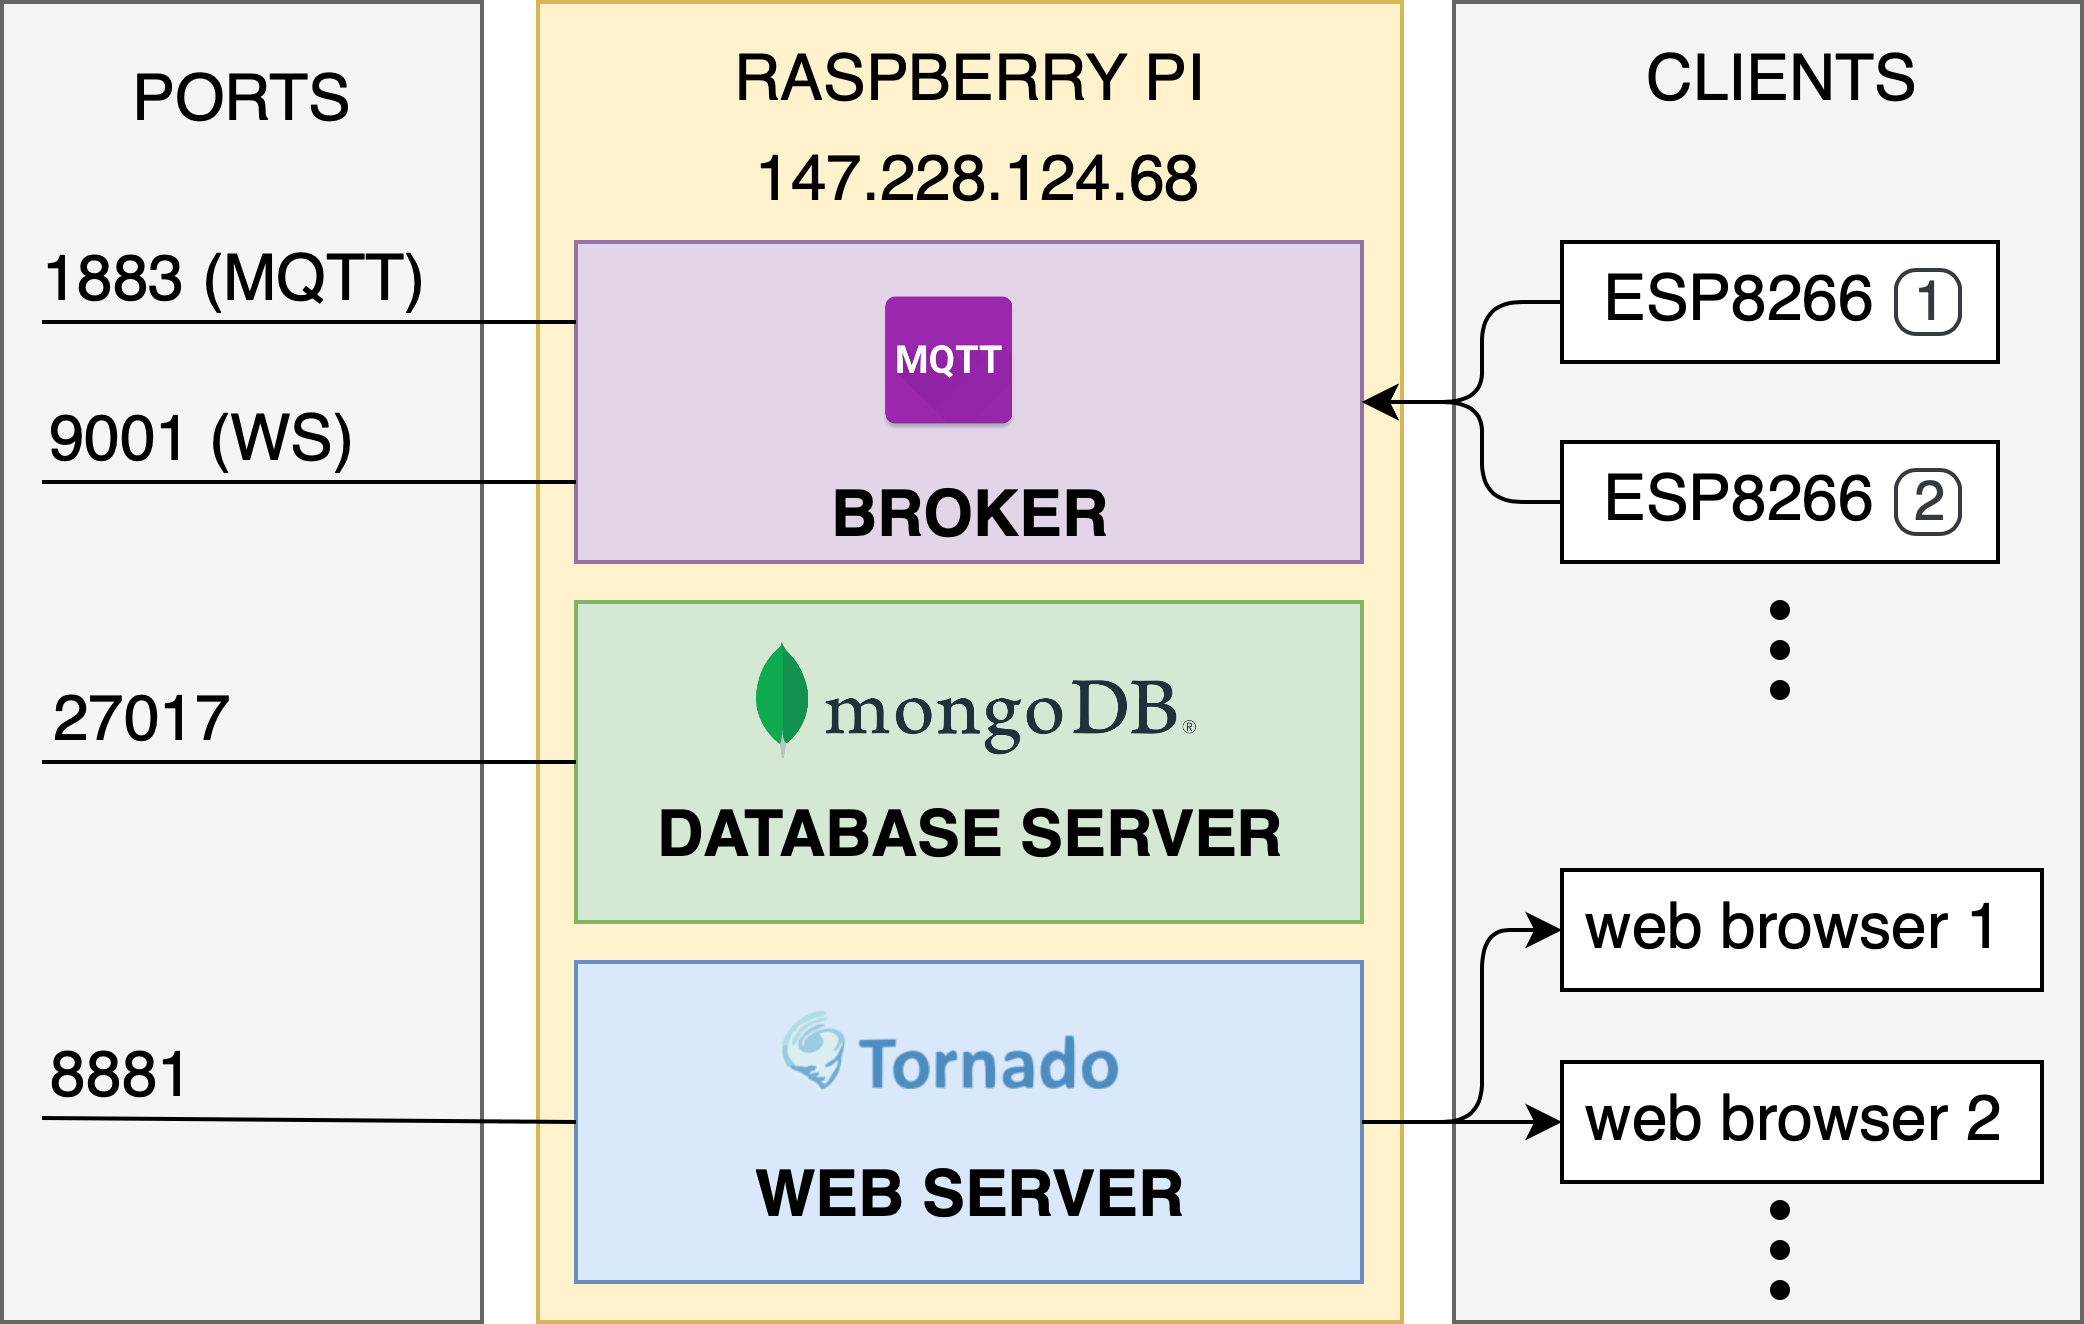
\includegraphics[width=0.6 \textwidth]{rpi_ports.png}
  \caption{Schéma procesů s popisy portů běžících na Raspberry Pi}
  \label{fig:rpi_ports}
\end{figure}

K zajištění všech těchto procesů je architektura kódu na RPi s využitím principů objektově orientovaného programování rozdělena do souborů \textit{engine.py, model.py, data.py, models.json, config.cfg}. Diagram architektury kódu s rozdělením do souborů je zobrazen na \cref{fig:backend_architecture}.

\begin{figure}[H]
  \centering
  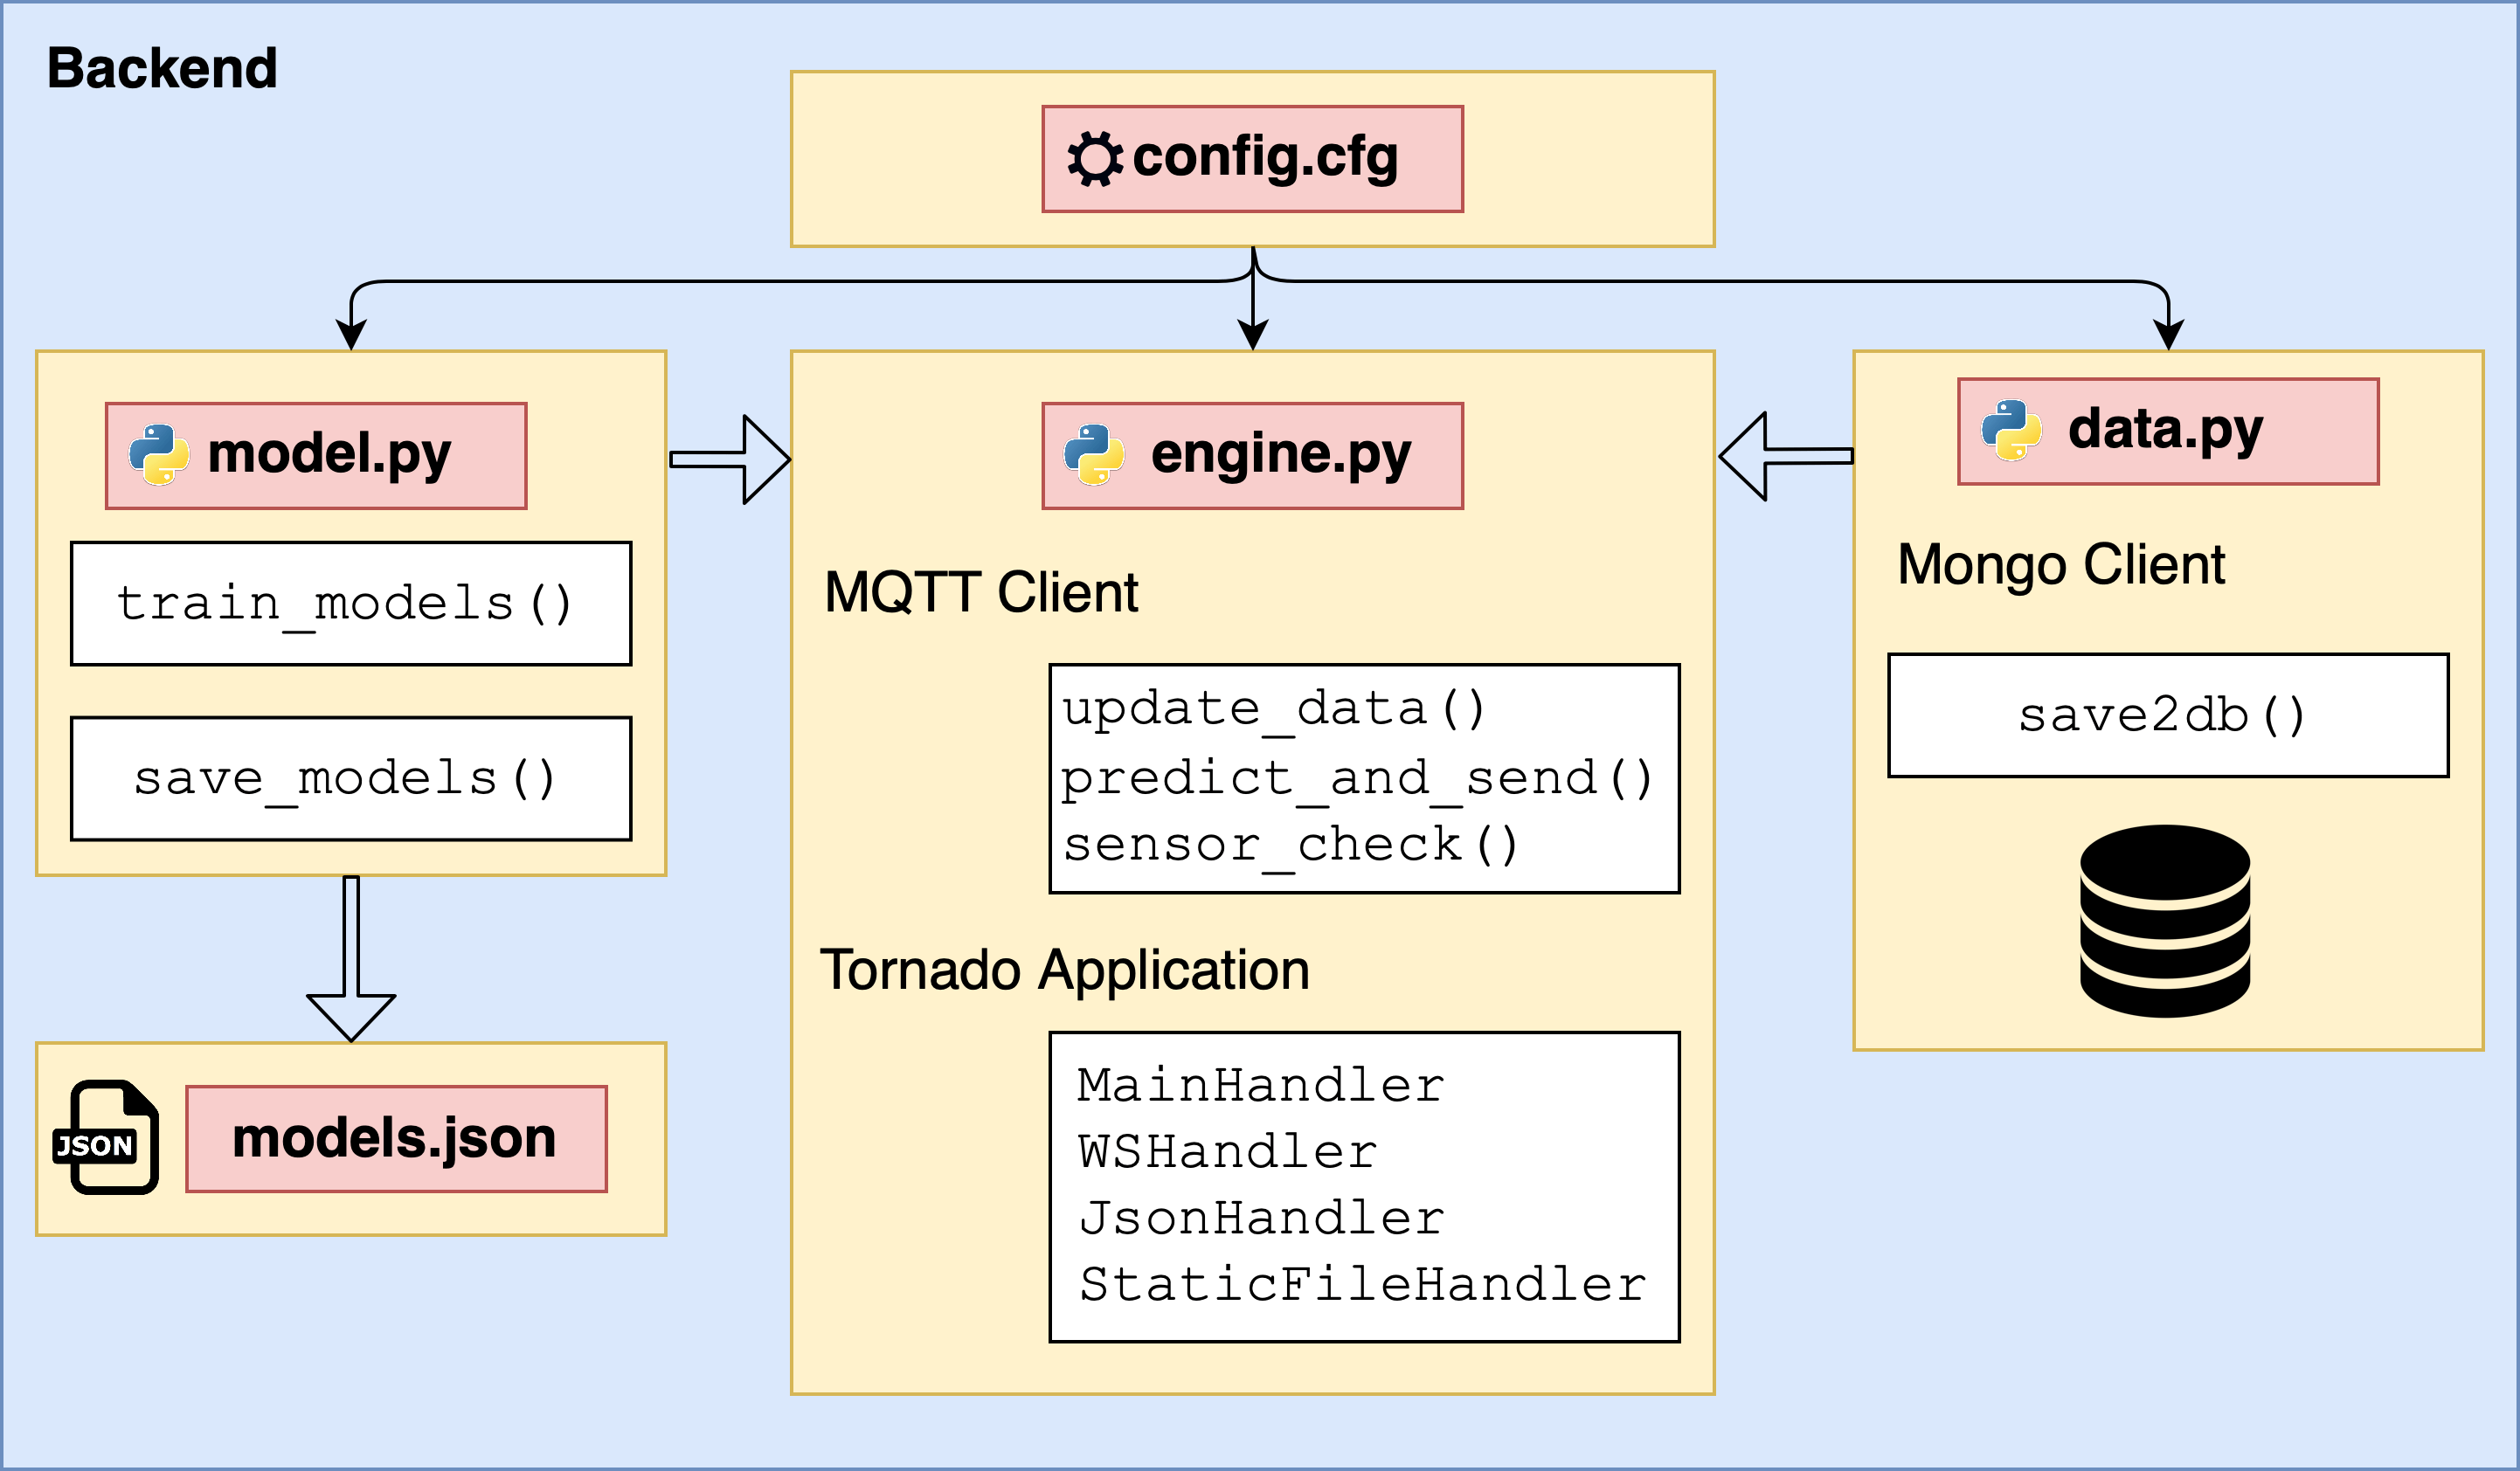
\includegraphics[width=0.8 \textwidth]{backend_architecture.png}
  \caption{Diagram architektury kódu backendu na Raspberry Pi}
  \label{fig:backend_architecture}
\end{figure}

Nad všemi skripty je konfigurační soubor \textit{config.cfg} se vstupními parametry. Konfigurační soubor obsahuje parametry pro připojení k MQTT brokeru, porty pro webový a databázový server a parametry pro trénování modelů. \textit{Engine.py} je hlavní skript, který využívá metod ze skriptů \textit{model.py} a \textit{data.py}. Funkce pro ukládání všech příchozích zpráv do databáze jsou nadefinovány ve skriptu data.py. V tomto skriptu je vytvořena instance objektu \textit{MongoClient} se vstupními parametry (název hosta a port). Jelikož databázový server (MongoDB) a webový server (jehož součástí je script data.py) běží fyzicky na stejném RPi, je název hosta "localhost" \ a výchozí port pro MongoDB je 27017. Hodnoty atributů ze zpráv jsou v databázi ukládány do kolekcí podle názvu topicu. Ve skriptu model.py probíhá trénování modelů pro predikci a klasifikaci naměřených hodnot (více v \cref{sec:classifier}). Skript model.py pracuje se souborem \textit{model.json}, ve kterém jsou uloženy parametry pro trénování modelů - například časové období od kdy do kdy jsou brány vzorky dat pro trénování modelu. Skript engine.py se skládá ze dvou hlavních částí - MQTT Client a Tornado Application. Ve třídě MQTT Client jsou odebírána data z brokeru, tato data jsou klasifikována a následně přes Websocket odesílána na webovou stránku. Třída Tornado Application je tvořena několika "Handlery". \textit{MainHandler} se stará o renderování webové stránky - zpřístupňuje webovou stránku pod IP adresou ve webovém prohlížeči. Třída \textit{WSHandler} obstarává komunikaci mezi webovým prohlížečem a serverem (např.: když uživatel volí, který model chce zobrazit). \textit{JsonHandler} je třída, která pracuje s json soubory v backendové části serveru. Tento handler je využitý k propagaci denních statistik natrénovaných klasifikátorů (denní statistika je zobrazena např.: na \cref{fig:web_analytics1}). Tyto statistiky se nahrávají na web pouze jednou při načtení webové stránky, proto není nutné používat protokol Websocket. Vhodnější je využití json souboru, se kterým pracuje JsonHandler.

\subsection*{Websocket} \label{sec:websocket}
\textit{Websocket} je síťový komunikační protokol, který umožňuje obousměrnou komunikaci po TCP protokolu. Jedná se o protokol, který má využití především ve webových aplikacích při komunikaci mezi klientem a serverem. V projektu chytré domácnosti je tento protokol využíván pro komunikaci mezi serverem a webovou vizualizací. Webová stránka potřebuje neustále aktuální data (naměřené hodnoty veličin) ze senzorů. Websocket je ideální řešení přenosu dat ze serveru do webového klienta v reálném čase s minimální výpočetní náročností. Ve chvíli, kdy na broker přijde nová zpráva, je tato zpráva ihned odeslána protokolem Websocket na webového klienta a webová stránka zobrazuje neustále aktuální data bez nutnosti obnovy stránky. Alternativou tohoto protokolu může být například načítání dat z externího souboru. Je možné vytvořit json soubor, do kterého budou nově příchozí zprávy ukládány a webová stránka bude periodicky načítat data z tohoto souboru. Hlavní nevýhodou tohoto přístupu je nutnost periodické kontroly externího souboru s daty. K tomu, aby na webové stránce byla neustále aktuální data, by bylo potřeba načítat soubor velmi často - například každé 2 až 3 vteřiny. To je velmi neefektivní, protože nová data ze senzoru chodí pravidelně po 1 minutě. Webový klient by tedy pořád otevíral soubor s daty a kontroloval, zda v něm jsou nová data, přičemž u naprosté většiny těchto kontrol by zjistil, že data jsou stále stejná. Tuto neefektivitu a zbytečnou výpočetní složitost nahrazuje protokol Websocket. Zásadní výhodou protokolu Websocket je možnost odesílání dat ze serveru do webového prohlížeče, aniž by si klient tuto zprávu musel vyžádat (tj. klient se nemusí každé 2-3 vteřiny dotazovat serveru zda nemá nová data. Nová data dostane automaticky ve chvíli, kdy je server obdrží). Současně je možné využít Websocket i pro komunikaci opačným směrem - z klienta na server a uživateli tím umožnit interagovat s daty v backendu prostřednictvím webového prohlížeče. Tento směr komunikace lze využít například pro přetrénování modelů na základě vstupních parametrů, které uživatel zadá na webové stránce (uživatel může měnit časové rozpětí dat - od kdy do kdy, která jsou použita pro trénování modelu).